\documentclass{article}
\usepackage{amsmath,amssymb,amsthm,mathtools}
\usepackage{tikz-cd}

\begin{document}

\title{Issue XXV: Caregory Theory}
\author{Максим Сохацький $^1$}
\date{ $^1$ Національний технічний університет України \\
       \small Київський політехнічний інститут імені Ігоря Сікорського \\
       \today }
\maketitle

\begin{abstract}

Formal definition of Category.

{\bf Keywords}: Category Theory \\
\end{abstract}

\ifincludeTOC
  \tableofcontents
\fi

\section{Category Theory}

\subsection{Category}

First of all very simple category theory up to pullbacks is provided. We give here
all definitions only to keep the context valid.

A \textbf{category} $\mathcal{C}$ consists of:
\begin{itemize}
  \item A class of \textbf{objects}, $\mathrm{Ob}(\mathcal{C})$,
  \item A class of \textbf{morphisms}, $\mathrm{Hom}_{\mathcal{C}}(X,Y)$, for each pair $X,Y \in \mathrm{Ob}(\mathcal{C})$,
  \item Composition maps $\circ: \mathrm{Hom}(Y,Z) \times \mathrm{Hom}(X,Y) \to \mathrm{Hom}(X,Z)$,
  \item Identity morphisms $\mathrm{id}_X \in \mathrm{Hom}(X,X)$ for each $X$,
\end{itemize}
satisfying associativity and identity laws.

\begin{definition} (Category Signature). The signature of category is
a $\sum_{A:U}A \rightarrow A \rightarrow U$ where $U$ could be any universe.
The $\mathrm{pr}_1$ projection is called $\mathrm{Ob}$ and $\mathrm{pr}_2$ projection is
called $\mathrm{Hom}(a,b)$, where $a,b:\mathrm{Ob}$.
\begin{lstlisting}
cat: U = (A: U) * (A -> A -> U)
\end{lstlisting}
\end{definition}

\begin{definition} (Precategory). More formal, precategory $\mathrm{C}$ consists of the following.
(i) A type $\mathrm{Ob}_C$, whose elements are called objects;
(ii) for each $a,b: \mathrm{Ob}_C$, a set $\mathrm{Hom}_C(a,b)$, whose elements are called arrows or morphisms.
(iii) For each $a: \mathrm{Ob}_C$, a morphism $1_a : \mathrm{Hom}_C(a,a)$, called the identity morphism.
(iv) For each $a,b,c: \mathrm{Ob}_C$, a function
     $\mathrm{Hom}_C(b,c) \rightarrow \mathrm{Hom}_C(a,b) \rightarrow \mathrm{Hom}_C(a,c)$
     called composition, and denoted $g \circ f$.
(v) For each $a,b: \mathrm{Ob}_C$ and $f: \mathrm{Hom}_C(a,b)$, $f = 1_b \circ f$ and $f = f \circ 1_a$.
(vi) For each $a,b,c,d: A$ and $f: \mathrm{Hom}_C(a,b)$, $g: \mathrm{Hom}_C(b,c)$, $h: \mathrm{Hom}_C(c,d)$,
     $h \circ (g \circ f ) = (h \circ g) \circ f$.
\begin{lstlisting}
isPrecategory (C: cat): U
  = (id: (x: C.1) -> C.2 x x)
  * (c: (x y z: C.1) -> C.2 x y -> C.2 y z -> C.2 x z)
  * (homSet: (x y: C.1) -> isSet (C.2 x y))
  * (left: (x y: C.1) -> (f: C.2 x y) ->
    Path (C.2 x y) (c x x y (id x) f) f)
  * (right: (x y: C.1) -> (f: C.2 x y) ->
    Path (C.2 x y) (c x y y f (id y)) f)
  * ( (x y z w: C.1) -> (f: C.2 x y) ->
    (g: C.2 y z) -> (h: C.2 z w) ->
    Path (C.2 x w) (c x z w (c x y z f g) h)
                   (c x y w f (c y z w g h)))
\end{lstlisting}
\begin{lstlisting}
carrier (C: precategory) : U
hom     (C: precategory) (a b: carrier C) : U
compose (C: precategory) (x y z: carrier C)
        (f: hom C x y) (g: hom C y z) : hom C x z
\end{lstlisting}
\end{definition}

\subsection{Pullback}

\begin{definition} (Categorical Pullback).
The pullback of the cospan $A \mapright{f} C \mapleft{g} B$ is a object $A \times_{C} B$ with
morphisms $pb_1 : \times_C \rightarrow A $, $pb_2 : \times_C \rightarrow B$, such that
diagram commutes:
\begin{center}
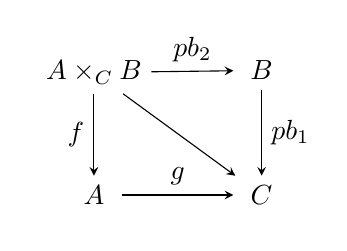
\begin{tikzpicture}
  \matrix (m) [matrix of math nodes,row sep=3em,column sep=3em,minimum width=2em]
  {
     A \times_{C} B & B \\
     A & C\\};
  \path[-stealth]
    (m-1-1) edge node [above] {$pb_2$} (m-1-2)
            edge node [above] {$$} (m-2-2)
    (m-1-1) edge node [left]  {$f$} (m-2-1)
    (m-1-2) edge node [right] {$pb_1$} (m-2-2)
    (m-2-1) edge node [above] {$g$} (m-2-2);
\end{tikzpicture}
\end{center}
Pullback $(\times_C,pb_1,pb_2)$ must be universal, means for any $(D,q_1,q_2)$
for which diagram also commutes there must exists a unique $u: D \rightarrow \times_C$,
such that $pb_1 \circ u = q_1$ and $pb_2 \circ q_2$.
\begin{lstlisting}
homTo  (C: precategory) (X: carrier C): U
  = (Y: carrier C) * hom C Y X
cospan (C: precategory): U
  = (X: carrier C) * (_: homTo C X) * homTo C X
cospanCone (C: precategory) (D: cospan C): U
  = (W: carrier C) * hasCospanCone C D W
cospanConeHom (C: precategory) (D: cospan C)
    (E1 E2: cospanCone C D) : U
  = (h: hom C E1.1 E2.1) * isCospanConeHom C D E1 E2 h
isPullback (C: precategory) (D: cospan C) (E: cospanCone C D) : U
  = (h: cospanCone C D) -> isContr (cospanConeHom C D h E)
hasPullback (C: precategory) (D: cospan C) : U
  = (E: cospanCone C D) * isPullback C D E
\end{lstlisting}
\end{definition}

\subsection{Functor}

A \textbf{functor} $F: \mathcal{C} \to \mathcal{D}$ assigns to each:
\begin{itemize}
  \item Object $X \in \mathcal{C}$ an object $F(X) \in \mathcal{D}$,
  \item Morphism $f: X \to Y$ a morphism $F(f): F(X) \to F(Y)$,
\end{itemize}
such that $F(\mathrm{id}_X) = \mathrm{id}_{F(X)}$ and $F(g \circ f) = F(g) \circ F(f)$.


\begin{definition} (Category Functor).
Let $A$ and $B$ be precategories.
A functor $F : A \rightarrow B$ consists of: (i) A function $F_{Ob}: Ob_hA \rightarrow Ob_B$;
(ii) for each $a,b:Ob_A$, a function $F_{Hom}:Hom_A(a,b)\rightarrow Hom_B(F_{Ob}(a),F_{Ob}(b))$;
(iii) for each $a:Ob_A$, $F_{Ob}(1_a) = 1_{F_{Ob}}(a)$;
(iv) for $a,b,c:Ob_A$ and $f: Hom_A(a,b)$ and $g: Hom_A(b,c)$, $F(g\circ f) = F_{Hom}(g)\circ F_{Hom}(f)$.
\begin{lstlisting}
catfunctor (A B: precategory): U
  = (ob: carrier A -> carrier B)
  * (mor: (x y:carrier A)->hom A x y->hom B(ob x)(ob y))
  * (id: (x: carrier A) -> Path (hom B (ob x) (ob x))
    (mor x x (path A x)) (path B (ob x)))
  * ((x y z: carrier A) -> (f: hom A x y) -> (g: hom A y z) ->
    Path (hom B (ob x) (ob z)) (mor x z (compose A x y z f g))
         (compose B (ob x) (ob y) (ob z) (mor x y f) (mor y z g)))
\end{lstlisting}
\end{definition}

\newpage
\begin{definition} (Terminal Object). Is such object $\mathrm{Ob}_C$,
that
$$
    \prod_{x,y:\mathrm{Ob}_C} \mathrm{isContr} (\mathrm{Hom}_C(y,x)).
$$
\begin{lstlisting}
isTerminal (C: precategory) (y: carrier C): U
  = (x: carrier C) -> isContr (hom C x y)
terminal (C: precategory): U
  = (y: carrier C) * isTerminal C y
\end{lstlisting}
\end{definition}

\subsection{Natural Transformation}
A \textbf{natural transformation} $\eta: F \Rightarrow G$ between functors $F, G: \mathcal{C} \to \mathcal{D}$ consists of morphisms $\eta_X: F(X) \to G(X)$ such that for every $f: X \to Y$ in $\mathcal{C}$,
\[
\begin{tikzcd}
F(X) \arrow[r, "\eta_X"] \arrow[d, "F(f)"'] & G(X) \arrow[d, "G(f)"] \\
F(Y) \arrow[r, "\eta_Y"'] & G(Y)
\end{tikzcd}
\]
commutes.

\subsection{Adjunction}
An \textbf{adjunction} between categories $\mathcal{C}$ and $\mathcal{D}$ consists of functors
\[
F: \mathcal{C} \leftrightarrows \mathcal{D} : G
\]
and natural transformations (unit $\eta$ and counit $\varepsilon$)
\[
\eta: \mathrm{Id}_{\mathcal{C}} \Rightarrow G \circ F, \quad \varepsilon: F \circ G \Rightarrow \mathrm{Id}_{\mathcal{D}}
\]
satisfying the triangle identities.

%\begin{definition}
%\begin{lstlisting}
%\end{lstlisting}
%\end{definition}

\end{document}
